\documentclass[1p]{elsarticle_modified}
%\bibliographystyle{elsarticle-num}

%\usepackage[colorlinks]{hyperref}
%\usepackage{abbrmath_seonhwa} %\Abb, \Ascr, \Acal ,\Abf, \Afrak
\usepackage{amsfonts}
\usepackage{amssymb}
\usepackage{amsmath}
\usepackage{amsthm}
\usepackage{scalefnt}
\usepackage{amsbsy}
\usepackage{kotex}
\usepackage{caption}
\usepackage{subfig}
\usepackage{color}
\usepackage{graphicx}
\usepackage{xcolor} %% white, black, red, green, blue, cyan, magenta, yellow
\usepackage{float}
\usepackage{setspace}
\usepackage{hyperref}

\usepackage{tikz}
\usetikzlibrary{arrows}

\usepackage{multirow}
\usepackage{array} % fixed length table
\usepackage{hhline}

%%%%%%%%%%%%%%%%%%%%%
\makeatletter
\renewcommand*\env@matrix[1][\arraystretch]{%
	\edef\arraystretch{#1}%
	\hskip -\arraycolsep
	\let\@ifnextchar\new@ifnextchar
	\array{*\c@MaxMatrixCols c}}
\makeatother %https://tex.stackexchange.com/questions/14071/how-can-i-increase-the-line-spacing-in-a-matrix
%%%%%%%%%%%%%%%

\usepackage[normalem]{ulem}

\newcommand{\msout}[1]{\ifmmode\text{\sout{\ensuremath{#1}}}\else\sout{#1}\fi}
%SOURCE: \msout is \stkout macro in https://tex.stackexchange.com/questions/20609/strikeout-in-math-mode

\newcommand{\cancel}[1]{
	\ifmmode
	{\color{red}\msout{#1}}
	\else
	{\color{red}\sout{#1}}
	\fi
}

\newcommand{\add}[1]{
	{\color{blue}\uwave{#1}}
}

\newcommand{\replace}[2]{
	\ifmmode
	{\color{red}\msout{#1}}{\color{blue}\uwave{#2}}
	\else
	{\color{red}\sout{#1}}{\color{blue}\uwave{#2}}
	\fi
}

\newcommand{\Sol}{\mathcal{S}} %segment
\newcommand{\D}{D} %diagram
\newcommand{\A}{\mathcal{A}} %arc


%%%%%%%%%%%%%%%%%%%%%%%%%%%%%5 test

\def\sl{\operatorname{\textup{SL}}(2,\Cbb)}
\def\psl{\operatorname{\textup{PSL}}(2,\Cbb)}
\def\quan{\mkern 1mu \triangleright \mkern 1mu}

\theoremstyle{definition}
\newtheorem{thm}{Theorem}[section]
\newtheorem{prop}[thm]{Proposition}
\newtheorem{lem}[thm]{Lemma}
\newtheorem{ques}[thm]{Question}
\newtheorem{cor}[thm]{Corollary}
\newtheorem{defn}[thm]{Definition}
\newtheorem{exam}[thm]{Example}
\newtheorem{rmk}[thm]{Remark}
\newtheorem{alg}[thm]{Algorithm}

\newcommand{\I}{\sqrt{-1}}
\begin{document}

%\begin{frontmatter}
%
%\title{Boundary parabolic representations of knots up to 8 crossings}
%
%%% Group authors per affiliation:
%\author{Yunhi Cho} 
%\address{Department of Mathematics, University of Seoul, Seoul, Korea}
%\ead{yhcho@uos.ac.kr}
%
%
%\author{Seonhwa Kim} %\fnref{s_kim}}
%\address{Center for Geometry and Physics, Institute for Basic Science, Pohang, 37673, Korea}
%\ead{ryeona17@ibs.re.kr}
%
%\author{Hyuk Kim}
%\address{Department of Mathematical Sciences, Seoul National University, Seoul 08826, Korea}
%\ead{hyukkim@snu.ac.kr}
%
%\author{Seokbeom Yoon}
%\address{Department of Mathematical Sciences, Seoul National University, Seoul, 08826,  Korea}
%\ead{sbyoon15@snu.ac.kr}
%
%\begin{abstract}
%We find all boundary parabolic representation of knots up to 8 crossings.
%
%\end{abstract}
%\begin{keyword}
%    \MSC[2010] 57M25 
%\end{keyword}
%
%\end{frontmatter}

%\linenumbers
%\tableofcontents
%
\newcommand\colored[1]{\textcolor{white}{\rule[-0.35ex]{0.8em}{1.4ex}}\kern-0.8em\color{red} #1}%
%\newcommand\colored[1]{\textcolor{white}{ #1}\kern-2.17ex	\textcolor{white}{ #1}\kern-1.81ex	\textcolor{white}{ #1}\kern-2.15ex\color{red}#1	}

{\Large $\underline{11n_{68}~(K11n_{68})}$}

\setlength{\tabcolsep}{10pt}
\renewcommand{\arraystretch}{1.6}
\vspace{1cm}\begin{tabular}{m{100pt}>{\centering\arraybackslash}m{274pt}}
\multirow{5}{120pt}{
	\centering
	\includegraphics[width=112pt]{../../../GIT/diagram.site/Diagrams/png/684_11n_68.png}\\
\ \ \ A knot diagram\footnotemark}&
\allowdisplaybreaks
\textbf{Linearized knot diagam} \\
\cline{2-2}
 &
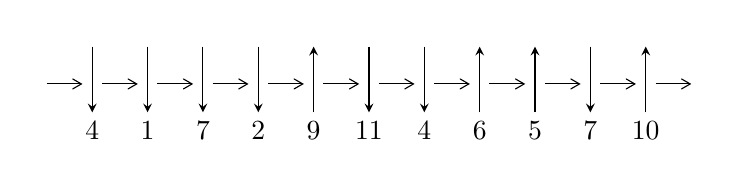
\begin{tikzpicture}[x=20pt, y=17pt]
	% nodes
	\node (C0) at (0, 0) {};
	\node (C1) at (1, 0) {};
	\node (C1U) at (1, +1) {};
	\node (C1D) at (1, -1) {4};

	\node (C2) at (2, 0) {};
	\node (C2U) at (2, +1) {};
	\node (C2D) at (2, -1) {1};

	\node (C3) at (3, 0) {};
	\node (C3U) at (3, +1) {};
	\node (C3D) at (3, -1) {7};

	\node (C4) at (4, 0) {};
	\node (C4U) at (4, +1) {};
	\node (C4D) at (4, -1) {2};

	\node (C5) at (5, 0) {};
	\node (C5U) at (5, +1) {};
	\node (C5D) at (5, -1) {9};

	\node (C6) at (6, 0) {};
	\node (C6U) at (6, +1) {};
	\node (C6D) at (6, -1) {11};

	\node (C7) at (7, 0) {};
	\node (C7U) at (7, +1) {};
	\node (C7D) at (7, -1) {4};

	\node (C8) at (8, 0) {};
	\node (C8U) at (8, +1) {};
	\node (C8D) at (8, -1) {6};

	\node (C9) at (9, 0) {};
	\node (C9U) at (9, +1) {};
	\node (C9D) at (9, -1) {5};

	\node (C10) at (10, 0) {};
	\node (C10U) at (10, +1) {};
	\node (C10D) at (10, -1) {7};

	\node (C11) at (11, 0) {};
	\node (C11U) at (11, +1) {};
	\node (C11D) at (11, -1) {10};
	\node (C12) at (12, 0) {};

	% arrows
	\draw[->,>={angle 60}]
	(C0) edge (C1) (C1) edge (C2) (C2) edge (C3) (C3) edge (C4) (C4) edge (C5) (C5) edge (C6) (C6) edge (C7) (C7) edge (C8) (C8) edge (C9) (C9) edge (C10) (C10) edge (C11) (C11) edge (C12) ;	\draw[->,>=stealth]
	(C1U) edge (C1D) (C2U) edge (C2D) (C3U) edge (C3D) (C4U) edge (C4D) (C5D) edge (C5U) (C6U) edge (C6D) (C7U) edge (C7D) (C8D) edge (C8U) (C9D) edge (C9U) (C10U) edge (C10D) (C11D) edge (C11U) ;
	\end{tikzpicture} \\
\hhline{~~} \\& 
\textbf{Solving Sequence} \\ \cline{2-2} 
 &
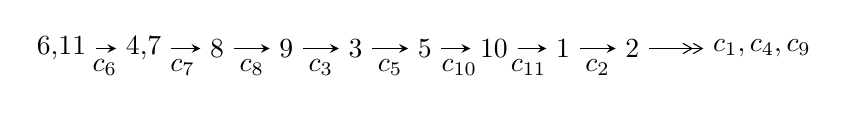
\begin{tikzpicture}[x=25pt, y=7pt]
	% node
	\node (A0) at (-1/8, 0) {6,11};
	\node (A1) at (17/16, 0) {4,7};
	\node (A2) at (17/8, 0) {8};
	\node (A3) at (25/8, 0) {9};
	\node (A4) at (33/8, 0) {3};
	\node (A5) at (41/8, 0) {5};
	\node (A6) at (49/8, 0) {10};
	\node (A7) at (57/8, 0) {1};
	\node (A8) at (65/8, 0) {2};
	\node (C1) at (1/2, -1) {$c_{6}$};
	\node (C2) at (13/8, -1) {$c_{7}$};
	\node (C3) at (21/8, -1) {$c_{8}$};
	\node (C4) at (29/8, -1) {$c_{3}$};
	\node (C5) at (37/8, -1) {$c_{5}$};
	\node (C6) at (45/8, -1) {$c_{10}$};
	\node (C7) at (53/8, -1) {$c_{11}$};
	\node (C8) at (61/8, -1) {$c_{2}$};
	\node (A9) at (10, 0) {$c_{1},c_{4},c_{9}$};

	% edge
	\draw[->,>=stealth]	
	(A0) edge (A1) (A1) edge (A2) (A2) edge (A3) (A3) edge (A4) (A4) edge (A5) (A5) edge (A6) (A6) edge (A7) (A7) edge (A8) ;
	\draw[->>,>={angle 60}]	
	(A8) edge (A9);
\end{tikzpicture} \\ 

\end{tabular} \\

\footnotetext{
The image of knot diagram is generated by the software ``\textbf{Draw programme}" developed by Andrew Bartholomew(\url{http://www.layer8.co.uk/maths/draw/index.htm\#Running-draw}), where we modified some parts for our purpose(\url{https://github.com/CATsTAILs/LinksPainter}).
}\phantom \\ \newline 
\centering \textbf{Ideals for irreducible components\footnotemark of $X_{\text{par}}$} 
 
\begin{align*}
I^u_{1}&=\langle 
77815 u^{25}-80433 u^{24}+\cdots+101496 b+29131,\\
\phantom{I^u_{1}}&\phantom{= \langle  }2049367 u^{25}+17170719 u^{24}+\cdots+12687000 a+47575387,\;u^{26}-2 u^{25}+\cdots-2 u+1\rangle \\
I^u_{2}&=\langle 
- u^3+2 b+u+1,\;- u^3-2 u^2+2 a-3 u-1,\;u^4+u^3+u^2+1\rangle \\
I^u_{3}&=\langle 
u^8- u^7+2 u^6- u^4+u^3- u^2+b- u,\;u^7+u^6+2 u^5+4 u^4+3 u^3+3 u^2+a+3 u+1,\\
\phantom{I^u_{3}}&\phantom{= \langle  }u^9+3 u^7+3 u^6+3 u^5+6 u^4+3 u^3+3 u^2+2 u-1\rangle \\
\\
\end{align*}
\raggedright * 3 irreducible components of $\dim_{\mathbb{C}}=0$, with total 39 representations.\\
\footnotetext{All coefficients of polynomials are rational numbers. But the coefficients are sometimes approximated in decimal forms when there is not enough margin.}
\newpage
\renewcommand{\arraystretch}{1}
\centering \section*{I. $I^u_{1}= \langle 77815 u^{25}-80433 u^{24}+\cdots+101496 b+29131,\;2.05\times10^{6} u^{25}+1.72\times10^{7} u^{24}+\cdots+1.27\times10^{7} a+4.76\times10^{7},\;u^{26}-2 u^{25}+\cdots-2 u+1 \rangle$}
\flushleft \textbf{(i) Arc colorings}\\
\begin{tabular}{m{7pt} m{180pt} m{7pt} m{180pt} }
\flushright $a_{6}=$&$\begin{pmatrix}1\\0\end{pmatrix}$ \\
\flushright $a_{11}=$&$\begin{pmatrix}0\\u\end{pmatrix}$ \\
\flushright $a_{4}=$&$\begin{pmatrix}-0.161533 u^{25}-1.35341 u^{24}+\cdots+4.59237 u-3.74993\\-0.766680 u^{25}+0.792475 u^{24}+\cdots-0.209299 u-0.287016\end{pmatrix}$ \\
\flushright $a_{7}=$&$\begin{pmatrix}1\\u^2\end{pmatrix}$ \\
\flushright $a_{8}=$&$\begin{pmatrix}-4.34995 u^{25}+8.30824 u^{24}+\cdots-11.2562 u+4.44452\\0.111927 u^{25}+1.17301 u^{24}+\cdots-2.00774 u+1.43931\end{pmatrix}$ \\
\flushright $a_{9}=$&$\begin{pmatrix}-4.23802 u^{25}+9.48125 u^{24}+\cdots-13.2639 u+5.88383\\0.111927 u^{25}+1.17301 u^{24}+\cdots-2.00774 u+1.43931\end{pmatrix}$ \\
\flushright $a_{3}=$&$\begin{pmatrix}0.236517 u^{25}-2.54906 u^{24}+\cdots+7.57449 u-5.71342\\-1.07634 u^{25}+1.55091 u^{24}+\cdots-1.40645 u+0.112537\end{pmatrix}$ \\
\flushright $a_{5}=$&$\begin{pmatrix}-2.44452 u^{25}+1.53910 u^{24}+\cdots+0.243519 u-3.36715\\-1.39686 u^{25}+1.36224 u^{24}+\cdots-1.66316 u-0.888073\end{pmatrix}$ \\
\flushright $a_{10}=$&$\begin{pmatrix}u\\u^3+u\end{pmatrix}$ \\
\flushright $a_{1}=$&$\begin{pmatrix}u^3\\u^5+u^3+u\end{pmatrix}$ \\
\flushright $a_{2}=$&$\begin{pmatrix}-0.889032 u^{25}-0.919202 u^{24}+\cdots+5.34807 u-4.99096\\-1.17523 u^{25}+0.972343 u^{24}+\cdots+0.156712 u-0.961125\end{pmatrix}$\\ \flushright $a_{2}=$&$\begin{pmatrix}-0.889032 u^{25}-0.919202 u^{24}+\cdots+5.34807 u-4.99096\\-1.17523 u^{25}+0.972343 u^{24}+\cdots+0.156712 u-0.961125\end{pmatrix}$\\&\end{tabular}
\flushleft \textbf{(ii) Obstruction class $= -1$}\\~\\
\flushleft \textbf{(iii) Cusp Shapes $= -\frac{48418177}{8458000} u^{25}+\frac{48940111}{8458000} u^{24}+\cdots-\frac{705789}{8458000} u-\frac{61013797}{8458000}$}\\~\\
\newpage\renewcommand{\arraystretch}{1}
\flushleft \textbf{(iv) u-Polynomials at the component}\newline \\
\begin{tabular}{m{50pt}|m{274pt}}
Crossings & \hspace{64pt}u-Polynomials at each crossing \\
\hline $$\begin{aligned}c_{1},c_{4}\end{aligned}$$&$\begin{aligned}
&u^{26}-2 u^{25}+\cdots-35 u+4
\end{aligned}$\\
\hline $$\begin{aligned}c_{2}\end{aligned}$$&$\begin{aligned}
&u^{26}+10 u^{25}+\cdots+481 u+16
\end{aligned}$\\
\hline $$\begin{aligned}c_{3},c_{7}\end{aligned}$$&$\begin{aligned}
&u^{26}-2 u^{25}+\cdots-112 u+64
\end{aligned}$\\
\hline $$\begin{aligned}c_{5},c_{8},c_{9}\end{aligned}$$&$\begin{aligned}
&u^{26}+2 u^{25}+\cdots+2 u+1
\end{aligned}$\\
\hline $$\begin{aligned}c_{6},c_{10}\end{aligned}$$&$\begin{aligned}
&u^{26}+2 u^{25}+\cdots+2 u+1
\end{aligned}$\\
\hline $$\begin{aligned}c_{11}\end{aligned}$$&$\begin{aligned}
&u^{26}-14 u^{25}+\cdots-4 u+1
\end{aligned}$\\
\hline
\end{tabular}\\~\\
\newpage\renewcommand{\arraystretch}{1}
\flushleft \textbf{(v) Riley Polynomials at the component}\newline \\
\begin{tabular}{m{50pt}|m{274pt}}
Crossings & \hspace{64pt}Riley Polynomials at each crossing \\
\hline $$\begin{aligned}c_{1},c_{4}\end{aligned}$$&$\begin{aligned}
&y^{26}-10 y^{25}+\cdots-481 y+16
\end{aligned}$\\
\hline $$\begin{aligned}c_{2}\end{aligned}$$&$\begin{aligned}
&y^{26}+14 y^{25}+\cdots-80993 y+256
\end{aligned}$\\
\hline $$\begin{aligned}c_{3},c_{7}\end{aligned}$$&$\begin{aligned}
&y^{26}+18 y^{25}+\cdots+70400 y+4096
\end{aligned}$\\
\hline $$\begin{aligned}c_{5},c_{8},c_{9}\end{aligned}$$&$\begin{aligned}
&y^{26}+22 y^{25}+\cdots+4 y+1
\end{aligned}$\\
\hline $$\begin{aligned}c_{6},c_{10}\end{aligned}$$&$\begin{aligned}
&y^{26}+14 y^{25}+\cdots+4 y+1
\end{aligned}$\\
\hline $$\begin{aligned}c_{11}\end{aligned}$$&$\begin{aligned}
&y^{26}-2 y^{25}+\cdots+20 y+1
\end{aligned}$\\
\hline
\end{tabular}\\~\\
\newpage\flushleft \textbf{(vi) Complex Volumes and Cusp Shapes}
$$\begin{array}{c|c|c}  
\text{Solutions to }I^u_{1}& \I (\text{vol} + \sqrt{-1}CS) & \text{Cusp shape}\\
 \hline 
\begin{aligned}
u &= \phantom{-}1.011190 + 0.136706 I \\
a &= \phantom{-}0.035883 + 0.146636 I \\
b &= -0.62158 + 1.42798 I\end{aligned}
 & -1.86313 + 7.71246 I & -6.86228 - 5.25734 I \\ \hline\begin{aligned}
u &= \phantom{-}1.011190 - 0.136706 I \\
a &= \phantom{-}0.035883 - 0.146636 I \\
b &= -0.62158 - 1.42798 I\end{aligned}
 & -1.86313 - 7.71246 I & -6.86228 + 5.25734 I \\ \hline\begin{aligned}
u &= -0.370532 + 0.998437 I \\
a &= \phantom{-}1.109240 - 0.521057 I \\
b &= \phantom{-}0.369770 - 0.293138 I\end{aligned}
 & -2.47557 + 4.95345 I & -6.39722 - 7.47760 I \\ \hline\begin{aligned}
u &= -0.370532 - 0.998437 I \\
a &= \phantom{-}1.109240 + 0.521057 I \\
b &= \phantom{-}0.369770 + 0.293138 I\end{aligned}
 & -2.47557 - 4.95345 I & -6.39722 + 7.47760 I \\ \hline\begin{aligned}
u &= \phantom{-}0.269068 + 1.038770 I \\
a &= -0.127266 - 0.719999 I \\
b &= -0.463650 + 0.532995 I\end{aligned}
 & \phantom{-}1.31071 - 2.42285 I & \phantom{-}0.84038 + 4.76679 I \\ \hline\begin{aligned}
u &= \phantom{-}0.269068 - 1.038770 I \\
a &= -0.127266 + 0.719999 I \\
b &= -0.463650 - 0.532995 I\end{aligned}
 & \phantom{-}1.31071 + 2.42285 I & \phantom{-}0.84038 - 4.76679 I \\ \hline\begin{aligned}
u &= -0.132101 + 0.846386 I \\
a &= -0.69055 + 2.07222 I \\
b &= \phantom{-}1.30633 - 0.71384 I\end{aligned}
 & -0.911584 + 0.890121 I & \phantom{-}0.87423 + 1.36491 I \\ \hline\begin{aligned}
u &= -0.132101 - 0.846386 I \\
a &= -0.69055 - 2.07222 I \\
b &= \phantom{-}1.30633 + 0.71384 I\end{aligned}
 & -0.911584 - 0.890121 I & \phantom{-}0.87423 - 1.36491 I \\ \hline\begin{aligned}
u &= \phantom{-}0.330433 + 0.724477 I \\
a &= -0.95370 + 2.08665 I \\
b &= -1.142600 + 0.109328 I\end{aligned}
 & -5.04252 - 1.61304 I & -10.18355 + 3.58696 I \\ \hline\begin{aligned}
u &= \phantom{-}0.330433 - 0.724477 I \\
a &= -0.95370 - 2.08665 I \\
b &= -1.142600 - 0.109328 I\end{aligned}
 & -5.04252 + 1.61304 I & -10.18355 - 3.58696 I\\
 \hline 
 \end{array}$$\newpage$$\begin{array}{c|c|c}  
\text{Solutions to }I^u_{1}& \I (\text{vol} + \sqrt{-1}CS) & \text{Cusp shape}\\
 \hline 
\begin{aligned}
u &= \phantom{-}0.774839 + 0.143637 I \\
a &= \phantom{-}0.175331 - 0.241236 I \\
b &= \phantom{-}0.487210 + 1.045470 I\end{aligned}
 & \phantom{-}0.05851 - 2.13854 I & -4.58802 + 1.91237 I \\ \hline\begin{aligned}
u &= \phantom{-}0.774839 - 0.143637 I \\
a &= \phantom{-}0.175331 + 0.241236 I \\
b &= \phantom{-}0.487210 - 1.045470 I\end{aligned}
 & \phantom{-}0.05851 + 2.13854 I & -4.58802 - 1.91237 I \\ \hline\begin{aligned}
u &= \phantom{-}0.419572 + 0.612728 I \\
a &= -0.290716 - 0.333902 I \\
b &= \phantom{-}0.237389 + 0.425546 I\end{aligned}
 & -0.10620 - 1.46904 I & -0.77851 + 4.66825 I \\ \hline\begin{aligned}
u &= \phantom{-}0.419572 - 0.612728 I \\
a &= -0.290716 + 0.333902 I \\
b &= \phantom{-}0.237389 - 0.425546 I\end{aligned}
 & -0.10620 + 1.46904 I & -0.77851 - 4.66825 I \\ \hline\begin{aligned}
u &= -0.914066 + 0.917616 I \\
a &= \phantom{-}0.250251 + 0.130322 I \\
b &= \phantom{-}0.155646 + 0.140338 I\end{aligned}
 & -7.98517 + 3.33888 I & \phantom{-}1.72089 - 5.46783 I \\ \hline\begin{aligned}
u &= -0.914066 - 0.917616 I \\
a &= \phantom{-}0.250251 - 0.130322 I \\
b &= \phantom{-}0.155646 - 0.140338 I\end{aligned}
 & -7.98517 - 3.33888 I & \phantom{-}1.72089 + 5.46783 I \\ \hline\begin{aligned}
u &= \phantom{-}0.402493 + 1.239940 I \\
a &= \phantom{-}0.37826 - 1.94903 I \\
b &= \phantom{-}0.80677 + 1.32805 I\end{aligned}
 & \phantom{-}4.09462 - 6.26991 I & -1.96309 + 5.01662 I \\ \hline\begin{aligned}
u &= \phantom{-}0.402493 - 1.239940 I \\
a &= \phantom{-}0.37826 + 1.94903 I \\
b &= \phantom{-}0.80677 - 1.32805 I\end{aligned}
 & \phantom{-}4.09462 + 6.26991 I & -1.96309 - 5.01662 I \\ \hline\begin{aligned}
u &= -0.387462 + 1.292200 I \\
a &= -0.67996 - 1.61333 I \\
b &= -0.42179 + 1.55871 I\end{aligned}
 & \phantom{-}7.58035 + 1.64459 I & \phantom{-}1.58550 - 0.59315 I \\ \hline\begin{aligned}
u &= -0.387462 - 1.292200 I \\
a &= -0.67996 + 1.61333 I \\
b &= -0.42179 - 1.55871 I\end{aligned}
 & \phantom{-}7.58035 - 1.64459 I & \phantom{-}1.58550 + 0.59315 I\\
 \hline 
 \end{array}$$\newpage$$\begin{array}{c|c|c}  
\text{Solutions to }I^u_{1}& \I (\text{vol} + \sqrt{-1}CS) & \text{Cusp shape}\\
 \hline 
\begin{aligned}
u &= -0.553190 + 1.252930 I \\
a &= \phantom{-}0.89905 + 1.50339 I \\
b &= \phantom{-}0.43042 - 1.66549 I\end{aligned}
 & \phantom{-}6.35723 + 8.21738 I & -0.54202 - 5.78684 I \\ \hline\begin{aligned}
u &= -0.553190 - 1.252930 I \\
a &= \phantom{-}0.89905 - 1.50339 I \\
b &= \phantom{-}0.43042 + 1.66549 I\end{aligned}
 & \phantom{-}6.35723 - 8.21738 I & -0.54202 + 5.78684 I \\ \hline\begin{aligned}
u &= \phantom{-}0.560294 + 1.283400 I \\
a &= -0.58734 + 1.77218 I \\
b &= -0.96323 - 1.71069 I\end{aligned}
 & \phantom{-}1.68898 - 13.33640 I & -4.27120 + 7.69267 I \\ \hline\begin{aligned}
u &= \phantom{-}0.560294 - 1.283400 I \\
a &= -0.58734 - 1.77218 I \\
b &= -0.96323 + 1.71069 I\end{aligned}
 & \phantom{-}1.68898 + 13.33640 I & -4.27120 - 7.69267 I \\ \hline\begin{aligned}
u &= -0.410537 + 0.270705 I \\
a &= \phantom{-}0.73153 + 2.35210 I \\
b &= -0.430697 + 0.672525 I\end{aligned}
 & -4.35117 - 1.59149 I & -10.56012 + 0.81365 I \\ \hline\begin{aligned}
u &= -0.410537 - 0.270705 I \\
a &= \phantom{-}0.73153 - 2.35210 I \\
b &= -0.430697 - 0.672525 I\end{aligned}
 & -4.35117 + 1.59149 I & -10.56012 - 0.81365 I\\
 \hline 
 \end{array}$$\newpage\newpage\renewcommand{\arraystretch}{1}
\centering \section*{II. $I^u_{2}= \langle - u^3+2 b+u+1,\;- u^3-2 u^2+2 a-3 u-1,\;u^4+u^3+u^2+1 \rangle$}
\flushleft \textbf{(i) Arc colorings}\\
\begin{tabular}{m{7pt} m{180pt} m{7pt} m{180pt} }
\flushright $a_{6}=$&$\begin{pmatrix}1\\0\end{pmatrix}$ \\
\flushright $a_{11}=$&$\begin{pmatrix}0\\u\end{pmatrix}$ \\
\flushright $a_{4}=$&$\begin{pmatrix}\frac{1}{2} u^3+u^2+\frac{3}{2} u+\frac{1}{2}\\\frac{1}{2} u^3-\frac{1}{2} u-\frac{1}{2}\end{pmatrix}$ \\
\flushright $a_{7}=$&$\begin{pmatrix}1\\u^2\end{pmatrix}$ \\
\flushright $a_{8}=$&$\begin{pmatrix}1\\u^2\end{pmatrix}$ \\
\flushright $a_{9}=$&$\begin{pmatrix}u^2+1\\u^2\end{pmatrix}$ \\
\flushright $a_{3}=$&$\begin{pmatrix}\frac{1}{2} u^3+u^2+\frac{3}{2} u+\frac{1}{2}\\\frac{1}{2} u^3-\frac{1}{2} u-\frac{1}{2}\end{pmatrix}$ \\
\flushright $a_{5}=$&$\begin{pmatrix}- u^3\\- u^3- u^2-1\end{pmatrix}$ \\
\flushright $a_{10}=$&$\begin{pmatrix}u\\u^3+u\end{pmatrix}$ \\
\flushright $a_{1}=$&$\begin{pmatrix}u^3\\u^3+u^2+1\end{pmatrix}$ \\
\flushright $a_{2}=$&$\begin{pmatrix}\frac{3}{2} u^3+u^2+\frac{3}{2} u+\frac{1}{2}\\\frac{3}{2} u^3+u^2-\frac{1}{2} u+\frac{1}{2}\end{pmatrix}$\\ \flushright $a_{2}=$&$\begin{pmatrix}\frac{3}{2} u^3+u^2+\frac{3}{2} u+\frac{1}{2}\\\frac{3}{2} u^3+u^2-\frac{1}{2} u+\frac{1}{2}\end{pmatrix}$\\&\end{tabular}
\flushleft \textbf{(ii) Obstruction class $= 1$}\\~\\
\flushleft \textbf{(iii) Cusp Shapes $= \frac{1}{4} u^3+\frac{7}{2} u^2+\frac{23}{4} u-\frac{37}{4}$}\\~\\
\newpage\renewcommand{\arraystretch}{1}
\flushleft \textbf{(iv) u-Polynomials at the component}\newline \\
\begin{tabular}{m{50pt}|m{274pt}}
Crossings & \hspace{64pt}u-Polynomials at each crossing \\
\hline $$\begin{aligned}c_{1}\end{aligned}$$&$\begin{aligned}
&(u-1)^4
\end{aligned}$\\
\hline $$\begin{aligned}c_{2},c_{4}\end{aligned}$$&$\begin{aligned}
&(u+1)^4
\end{aligned}$\\
\hline $$\begin{aligned}c_{3},c_{7}\end{aligned}$$&$\begin{aligned}
&u^4
\end{aligned}$\\
\hline $$\begin{aligned}c_{5}\end{aligned}$$&$\begin{aligned}
&u^4+u^3+3 u^2+2 u+1
\end{aligned}$\\
\hline $$\begin{aligned}c_{6}\end{aligned}$$&$\begin{aligned}
&u^4+u^3+u^2+1
\end{aligned}$\\
\hline $$\begin{aligned}c_{8},c_{9},c_{11}\end{aligned}$$&$\begin{aligned}
&u^4- u^3+3 u^2-2 u+1
\end{aligned}$\\
\hline $$\begin{aligned}c_{10}\end{aligned}$$&$\begin{aligned}
&u^4- u^3+u^2+1
\end{aligned}$\\
\hline
\end{tabular}\\~\\
\newpage\renewcommand{\arraystretch}{1}
\flushleft \textbf{(v) Riley Polynomials at the component}\newline \\
\begin{tabular}{m{50pt}|m{274pt}}
Crossings & \hspace{64pt}Riley Polynomials at each crossing \\
\hline $$\begin{aligned}c_{1},c_{2},c_{4}\end{aligned}$$&$\begin{aligned}
&(y-1)^4
\end{aligned}$\\
\hline $$\begin{aligned}c_{3},c_{7}\end{aligned}$$&$\begin{aligned}
&y^4
\end{aligned}$\\
\hline $$\begin{aligned}c_{5},c_{8},c_{9}\\c_{11}\end{aligned}$$&$\begin{aligned}
&y^4+5 y^3+7 y^2+2 y+1
\end{aligned}$\\
\hline $$\begin{aligned}c_{6},c_{10}\end{aligned}$$&$\begin{aligned}
&y^4+y^3+3 y^2+2 y+1
\end{aligned}$\\
\hline
\end{tabular}\\~\\
\newpage\flushleft \textbf{(vi) Complex Volumes and Cusp Shapes}
$$\begin{array}{c|c|c}  
\text{Solutions to }I^u_{2}& \I (\text{vol} + \sqrt{-1}CS) & \text{Cusp shape}\\
 \hline 
\begin{aligned}
u &= \phantom{-}0.351808 + 0.720342 I \\
a &= \phantom{-}0.38053 + 1.53420 I \\
b &= -0.927958 - 0.413327 I\end{aligned}
 & -1.43393 - 1.41510 I & -8.73606 + 5.88934 I \\ \hline\begin{aligned}
u &= \phantom{-}0.351808 - 0.720342 I \\
a &= \phantom{-}0.38053 - 1.53420 I \\
b &= -0.927958 + 0.413327 I\end{aligned}
 & -1.43393 + 1.41510 I & -8.73606 - 5.88934 I \\ \hline\begin{aligned}
u &= -0.851808 + 0.911292 I \\
a &= -0.130534 + 0.427872 I \\
b &= \phantom{-}0.677958 + 0.157780 I\end{aligned}
 & -8.43568 + 3.16396 I & -14.13894 + 0.11292 I \\ \hline\begin{aligned}
u &= -0.851808 - 0.911292 I \\
a &= -0.130534 - 0.427872 I \\
b &= \phantom{-}0.677958 - 0.157780 I\end{aligned}
 & -8.43568 - 3.16396 I & -14.13894 - 0.11292 I\\
 \hline 
 \end{array}$$\newpage\newpage\renewcommand{\arraystretch}{1}
\centering \section*{III. $I^u_{3}= \langle u^8- u^7+2 u^6- u^4+u^3- u^2+b- u,\;u^7+u^6+2 u^5+4 u^4+3 u^3+3 u^2+a+3 u+1,\;u^9+3 u^7+\cdots+2 u-1 \rangle$}
\flushleft \textbf{(i) Arc colorings}\\
\begin{tabular}{m{7pt} m{180pt} m{7pt} m{180pt} }
\flushright $a_{6}=$&$\begin{pmatrix}1\\0\end{pmatrix}$ \\
\flushright $a_{11}=$&$\begin{pmatrix}0\\u\end{pmatrix}$ \\
\flushright $a_{4}=$&$\begin{pmatrix}- u^7- u^6-2 u^5-4 u^4-3 u^3-3 u^2-3 u-1\\- u^8+u^7-2 u^6+u^4- u^3+u^2+u\end{pmatrix}$ \\
\flushright $a_{7}=$&$\begin{pmatrix}1\\u^2\end{pmatrix}$ \\
\flushright $a_{8}=$&$\begin{pmatrix}- u\\u\end{pmatrix}$ \\
\flushright $a_{9}=$&$\begin{pmatrix}0\\u\end{pmatrix}$ \\
\flushright $a_{3}=$&$\begin{pmatrix}- u^7-2 u^6-2 u^5-6 u^4-4 u^3-4 u^2-4 u\\-2 u^8+u^7-4 u^6- u^5-2 u^3+2 u^2+u\end{pmatrix}$ \\
\flushright $a_{5}=$&$\begin{pmatrix}1\\u^2\end{pmatrix}$ \\
\flushright $a_{10}=$&$\begin{pmatrix}u\\u^3+u\end{pmatrix}$ \\
\flushright $a_{1}=$&$\begin{pmatrix}u^3\\u^5+u^3+u\end{pmatrix}$ \\
\flushright $a_{2}=$&$\begin{pmatrix}- u^4- u^2-2 u-1\\u^4+2 u\end{pmatrix}$\\ \flushright $a_{2}=$&$\begin{pmatrix}- u^4- u^2-2 u-1\\u^4+2 u\end{pmatrix}$\\&\end{tabular}
\flushleft \textbf{(ii) Obstruction class $= -1$}\\~\\
\flushleft \textbf{(iii) Cusp Shapes $= -4 u^6-8 u^4-8 u^3-4 u^2-8 u-6$}\\~\\
\newpage\renewcommand{\arraystretch}{1}
\flushleft \textbf{(iv) u-Polynomials at the component}\newline \\
\begin{tabular}{m{50pt}|m{274pt}}
Crossings & \hspace{64pt}u-Polynomials at each crossing \\
\hline $$\begin{aligned}c_{1},c_{4}\end{aligned}$$&$\begin{aligned}
&(u^3- u^2+1)^3
\end{aligned}$\\
\hline $$\begin{aligned}c_{2},c_{3},c_{7}\end{aligned}$$&$\begin{aligned}
&(u^3+u^2+2 u+1)^3
\end{aligned}$\\
\hline $$\begin{aligned}c_{5},c_{6},c_{8}\\c_{9},c_{10}\end{aligned}$$&$\begin{aligned}
&u^9+3 u^7-3 u^6+3 u^5-6 u^4+3 u^3-3 u^2+2 u+1
\end{aligned}$\\
\hline $$\begin{aligned}c_{11}\end{aligned}$$&$\begin{aligned}
&u^9-6 u^8+15 u^7-15 u^6-5 u^5+24 u^4-9 u^3-15 u^2+10 u+1
\end{aligned}$\\
\hline
\end{tabular}\\~\\
\newpage\renewcommand{\arraystretch}{1}
\flushleft \textbf{(v) Riley Polynomials at the component}\newline \\
\begin{tabular}{m{50pt}|m{274pt}}
Crossings & \hspace{64pt}Riley Polynomials at each crossing \\
\hline $$\begin{aligned}c_{1},c_{4}\end{aligned}$$&$\begin{aligned}
&(y^3- y^2+2 y-1)^3
\end{aligned}$\\
\hline $$\begin{aligned}c_{2},c_{3},c_{7}\end{aligned}$$&$\begin{aligned}
&(y^3+3 y^2+2 y-1)^3
\end{aligned}$\\
\hline $$\begin{aligned}c_{5},c_{6},c_{8}\\c_{9},c_{10}\end{aligned}$$&$\begin{aligned}
&y^9+6 y^8+15 y^7+15 y^6-5 y^5-24 y^4-9 y^3+15 y^2+10 y-1
\end{aligned}$\\
\hline $$\begin{aligned}c_{11}\end{aligned}$$&$\begin{aligned}
&y^9-6 y^8+\cdots+130 y-1
\end{aligned}$\\
\hline
\end{tabular}\\~\\
\newpage\flushleft \textbf{(vi) Complex Volumes and Cusp Shapes}
$$\begin{array}{c|c|c}  
\text{Solutions to }I^u_{3}& \I (\text{vol} + \sqrt{-1}CS) & \text{Cusp shape}\\
 \hline 
\begin{aligned}
u &= -0.149100 + 1.032810 I \\
a &= -1.49322 - 1.81245 I \\
b &= \phantom{-}1.57125 + 2.35293 I\end{aligned}
 & -1.11345\phantom{ +0.000000I} & -9.01951 + 0. I\phantom{ +0.000000I} \\ \hline\begin{aligned}
u &= -0.149100 - 1.032810 I \\
a &= -1.49322 + 1.81245 I \\
b &= \phantom{-}1.57125 - 2.35293 I\end{aligned}
 & -1.11345\phantom{ +0.000000I} & -9.01951 + 0. I\phantom{ +0.000000I} \\ \hline\begin{aligned}
u &= -0.929255 + 0.157692 I \\
a &= -0.1261290 + 0.0333681 I \\
b &= \phantom{-}0.119081 + 1.372090 I\end{aligned}
 & \phantom{-}3.02413 - 2.82812 I & -2.49024 + 2.97945 I \\ \hline\begin{aligned}
u &= -0.929255 - 0.157692 I \\
a &= -0.1261290 - 0.0333681 I \\
b &= \phantom{-}0.119081 - 1.372090 I\end{aligned}
 & \phantom{-}3.02413 + 2.82812 I & -2.49024 - 2.97945 I \\ \hline\begin{aligned}
u &= \phantom{-}0.550542 + 1.200360 I \\
a &= -1.08414 + 1.00782 I \\
b &= \phantom{-}0.116542 - 1.272430 I\end{aligned}
 & \phantom{-}3.02413 - 2.82812 I & -2.49024 + 2.97945 I \\ \hline\begin{aligned}
u &= \phantom{-}0.550542 - 1.200360 I \\
a &= -1.08414 - 1.00782 I \\
b &= \phantom{-}0.116542 + 1.272430 I\end{aligned}
 & \phantom{-}3.02413 + 2.82812 I & -2.49024 - 2.97945 I \\ \hline\begin{aligned}
u &= \phantom{-}0.378713 + 1.358050 I \\
a &= \phantom{-}0.84258 - 1.19340 I \\
b &= \phantom{-}0.00950 + 1.58939 I\end{aligned}
 & \phantom{-}3.02413 + 2.82812 I & -2.49024 - 2.97945 I \\ \hline\begin{aligned}
u &= \phantom{-}0.378713 - 1.358050 I \\
a &= \phantom{-}0.84258 + 1.19340 I \\
b &= \phantom{-}0.00950 - 1.58939 I\end{aligned}
 & \phantom{-}3.02413 - 2.82812 I & -2.49024 + 2.97945 I \\ \hline\begin{aligned}
u &= \phantom{-}0.298201\phantom{ +0.000000I} \\
a &= -2.27818\phantom{ +0.000000I} \\
b &= \phantom{-}0.367256\phantom{ +0.000000I}\end{aligned}
 & -1.11345\phantom{ +0.000000I} & -9.01950\phantom{ +0.000000I}\\
 \hline 
 \end{array}$$\newpage
\newpage\renewcommand{\arraystretch}{1}
\centering \section*{ IV. u-Polynomials}
\begin{tabular}{m{50pt}|m{274pt}}
Crossings & \hspace{64pt}u-Polynomials at each crossing \\
\hline $$\begin{aligned}c_{1}\end{aligned}$$&$\begin{aligned}
&((u-1)^4)(u^3- u^2+1)^3(u^{26}-2 u^{25}+\cdots-35 u+4)
\end{aligned}$\\
\hline $$\begin{aligned}c_{2}\end{aligned}$$&$\begin{aligned}
&((u+1)^4)(u^3+u^2+2 u+1)^3(u^{26}+10 u^{25}+\cdots+481 u+16)
\end{aligned}$\\
\hline $$\begin{aligned}c_{3},c_{7}\end{aligned}$$&$\begin{aligned}
&u^4(u^3+u^2+2 u+1)^3(u^{26}-2 u^{25}+\cdots-112 u+64)
\end{aligned}$\\
\hline $$\begin{aligned}c_{4}\end{aligned}$$&$\begin{aligned}
&((u+1)^4)(u^3- u^2+1)^3(u^{26}-2 u^{25}+\cdots-35 u+4)
\end{aligned}$\\
\hline $$\begin{aligned}c_{5}\end{aligned}$$&$\begin{aligned}
&(u^4+u^3+3 u^2+2 u+1)\\
&\cdot(u^9+3 u^7-3 u^6+3 u^5-6 u^4+3 u^3-3 u^2+2 u+1)\\
&\cdot(u^{26}+2 u^{25}+\cdots+2 u+1)
\end{aligned}$\\
\hline $$\begin{aligned}c_{6}\end{aligned}$$&$\begin{aligned}
&(u^4+u^3+u^2+1)(u^9+3 u^7-3 u^6+3 u^5-6 u^4+3 u^3-3 u^2+2 u+1)\\
&\cdot(u^{26}+2 u^{25}+\cdots+2 u+1)
\end{aligned}$\\
\hline $$\begin{aligned}c_{8},c_{9}\end{aligned}$$&$\begin{aligned}
&(u^4- u^3+3 u^2-2 u+1)\\
&\cdot(u^9+3 u^7-3 u^6+3 u^5-6 u^4+3 u^3-3 u^2+2 u+1)\\
&\cdot(u^{26}+2 u^{25}+\cdots+2 u+1)
\end{aligned}$\\
\hline $$\begin{aligned}c_{10}\end{aligned}$$&$\begin{aligned}
&(u^4- u^3+u^2+1)(u^9+3 u^7-3 u^6+3 u^5-6 u^4+3 u^3-3 u^2+2 u+1)\\
&\cdot(u^{26}+2 u^{25}+\cdots+2 u+1)
\end{aligned}$\\
\hline $$\begin{aligned}c_{11}\end{aligned}$$&$\begin{aligned}
&(u^4- u^3+3 u^2-2 u+1)\\
&\cdot(u^9-6 u^8+15 u^7-15 u^6-5 u^5+24 u^4-9 u^3-15 u^2+10 u+1)\\
&\cdot(u^{26}-14 u^{25}+\cdots-4 u+1)
\end{aligned}$\\
\hline
\end{tabular}\newpage\renewcommand{\arraystretch}{1}
\centering \section*{ V. Riley Polynomials}
\begin{tabular}{m{50pt}|m{274pt}}
Crossings & \hspace{64pt}Riley Polynomials at each crossing \\
\hline $$\begin{aligned}c_{1},c_{4}\end{aligned}$$&$\begin{aligned}
&((y-1)^4)(y^3- y^2+2 y-1)^3(y^{26}-10 y^{25}+\cdots-481 y+16)
\end{aligned}$\\
\hline $$\begin{aligned}c_{2}\end{aligned}$$&$\begin{aligned}
&((y-1)^4)(y^3+3 y^2+2 y-1)^3(y^{26}+14 y^{25}+\cdots-80993 y+256)
\end{aligned}$\\
\hline $$\begin{aligned}c_{3},c_{7}\end{aligned}$$&$\begin{aligned}
&y^4(y^3+3 y^2+2 y-1)^3(y^{26}+18 y^{25}+\cdots+70400 y+4096)
\end{aligned}$\\
\hline $$\begin{aligned}c_{5},c_{8},c_{9}\end{aligned}$$&$\begin{aligned}
&(y^4+5 y^3+7 y^2+2 y+1)\\
&\cdot(y^9+6 y^8+15 y^7+15 y^6-5 y^5-24 y^4-9 y^3+15 y^2+10 y-1)\\
&\cdot(y^{26}+22 y^{25}+\cdots+4 y+1)
\end{aligned}$\\
\hline $$\begin{aligned}c_{6},c_{10}\end{aligned}$$&$\begin{aligned}
&(y^4+y^3+3 y^2+2 y+1)\\
&\cdot(y^9+6 y^8+15 y^7+15 y^6-5 y^5-24 y^4-9 y^3+15 y^2+10 y-1)\\
&\cdot(y^{26}+14 y^{25}+\cdots+4 y+1)
\end{aligned}$\\
\hline $$\begin{aligned}c_{11}\end{aligned}$$&$\begin{aligned}
&(y^4+5 y^3+7 y^2+2 y+1)(y^9-6 y^8+\cdots+130 y-1)\\
&\cdot(y^{26}-2 y^{25}+\cdots+20 y+1)
\end{aligned}$\\
\hline
\end{tabular}
\vskip 2pc
\end{document}